\newpage
{\bfseries МРНТИ 52.13.07}
\hfill {\bfseries \href{https://doi.org/10.58805/kazutb.v.2.23-319}{https://doi.org/10.58805/kazutb.v.2.23-319}}

\sectionwithauthors{Д.К. Ахметканов, Л.Е. Тян, Е.Х. Абен, М. Елузах}{ОПТИМИЗАЦИЯ ЧИСЛЕННОСТИ И КАЧЕСТВЕННЫХ ХАРАКТЕРИСТИК ПОДЗЕМНОГО
ВЫЕМОЧНОГО ОБОРУДОВАНИЯ С ПРИМЕНЕНИЕМ ПРОГРАММНОГО ОБЕСПЕЧЕНИЯ
MICROMINE}

\begin{center}
{\bfseries Д.К. Ахметканов\envelope, Л.Е. Тян, Е.Х. Абен, М. Елузах}

Satbayev University, Алматы, Казахстан,

\envelope Корреспондент-автор:d.akhmetkanov@satbayev.university
\end{center}

В статье рассмотрено два варианта алгоритма оптимизации выемочных
единиц. В последние десятилетия угледобыча и добыча других полезных
ископаемых в подземных условиях стали сталкиваться с растущими вызовами,
такими как увеличение трудозатрат, изменение регулирования и постоянная
потребность в оптимизации процессов. В этом контексте внедрение
современных технологий, таких как программное обеспечение (ПО)
MICROMINE, предоставляет уникальные возможности для оптимизации
подземных выемочных добычных единиц. Оптимизатор выемочных единиц
определяет оптимальную комбинацию материнских блоков, которые необходимо
добыть, чтобы максимизировать общую прибыль от разработки месторождения.
При этом учитываются некоторые технологические ограничения. Если в
случае с оптимизацией открытых горных работ под технологическими
ограничениями подразумеваются углы откосов бортов карьеров, то при
оптимизации выемочных единиц учитываются минимальные размеры и форма
выемочных единиц. Экономический подход, сочетающий в себе уменьшение
затрат, увеличение добычи и минимизацию рисков, делает ПО MICROMINE
важным инструментом в индустрии добычи полезных ископаемых.

В данной работе целью является выявить алгоритм оптимизации подземных
выемочных единиц с применением ПО MICROMINE и выделить преимущества
использование данного программного обеспечения.

{\bfseries Ключевые слова:} оптимизация, выемочные единицы, блочная модель,
поперечное сечение, мощность, проектирование.

\begin{center}
{\large\bfseries MICROMINE БАҒДАРЛАМАЛЫҚ ЖАСАҚТАМАСЫН ҚОЛДАНА ОТЫРЫП, ЖЕРАСТЫ КЕН
ҚАЗУ ЖАБДЫҚТАРЫНЫҢ САНЫ МЕН САПАЛЫҚ СИПАТТАМАЛАРЫН ОҢТАЙЛАНДЫРУ}

{\bfseries Д.К. Ахметканов\envelope, Л.Е. Тян, Е.Х. Абен, М.
Елузах}

Сәтбаев Университеті, Алматы, Қазақстан,

е-mail: d.akhmetkanov@satbayev.university
\end{center}

Мақалада қазба бірліктерін оңтайландыру алгоритмінің екі нұсқасы
қарастырылған. Соңғы онжылдықтарда жерасты жағдайында көмір өндіру және
басқа да пайдалы қазбаларды игеруде еңбек шығындарының артуы, реттеудің
өзгеруі және процестерді оңтайландырудың тұрақты қажеттілігі сияқты өсіп
келе жатқан қиындықтарға тап болды. Осы тұрғыда MICROMINE бағдарламалық
жасақтамасы сияқты заманауи технологияларды енгізу жерасты кен игеру
өндірісін оңтайландырудың бірегей мүмкіндіктерін ұсынады. Қазба
бірліктерінің оңтайландырушысы кен орнын игеруден түскен жалпы пайданы
барынша арттыру үшін өндірілуге қажет аналық блоктардың оңтайлы
комбинациясын анықтайды. Бұл кейбір технологиялық шектеулерді ескереді.
Егер, ашық кен жұмыстарын оңтайландыру жағдайында технологиялық
шектеулер карьерлер бортының еңістерінің бұрыштарын білдірсе, онда қазба
бірліктерін оңтайландыру кезінде қазба бірліктерінің ең аз мөлшері мен
нысаны ескеріледі. Шығындарды азайтуды, өндірісті ұлғайтуды және
тәуекелдерді азайтуды біріктіретін Экономикалық тәсіл MICROMINE-ді
тау-кен өнеркәсібіндегі маңызды құралға айналдырады.

Бұл жұмыстың мақсаты MICROMINE бағдарламасының көмегімен жерасты кен
игерудегі қазу бірліктерін оңтайландыру алгоритмін анықтау және осы
бағдарламалық жасақтаманы пайдаланудың артықшылықтарын атап өту болып
табылады.

{\bfseries Түйін сөздер:} Оңтайландыру, кесу бірліктері, блоктық модель,
көлденең қима, қуат, жобалау.

\begin{center}
{\large\bfseries OPTIMIZATION OF THE NUMBER AND QUALITY CHARACTERISTICS OF
UNDERGROUND EXCAVATION EQUIPMENT USING MICROMINE SOFTWARE}

{\bfseries D. Akhmetkhanov\envelope, L. Tyan, E. Aben, M.
Eluzakh}

Satbayev University, Almaty, Kazakhstan,

е-mail: d.akhmetkanov@satbayev.university
\end{center}

The article considers two variants of the algorithm for optimizing
excavation units. In recent decades, coal mining and mining of other
minerals in underground conditions have begun to face growing
challenges, such as increased labor costs, regulatory changes and the
constant need to optimize processes. In this context, the introduction
of modern technologies such as MICROMINE software provides unique
opportunities for optimizing underground mining units. The dredging Unit
optimizer determines the optimal combination of parent blocks that need
to be mined in order to maximize the overall profit from the development
of the field. At the same time, some technological limitations are taken
into account. If, in the case of optimization of open-pit mining,
technological limitations mean the angles of the slopes of the sides of
quarries, then the minimum dimensions and shape of the excavation units
are taken into account when optimizing the excavation units. An economic
approach combining cost reduction, increased production and risk
minimization makes MICROMINE an important tool in the mining industry.

In this paper, the aim is to identify an algorithm for optimizing
underground excavation units using MICROMINE software and highlight the
advantages of using this software.

{\bfseries Keywords:} Optimization, excavation units, block model, cross
section, power, design.

\begin{multicols}{2}
{\bfseries Введение.} MICROMINE --- это интегрированное программное
обеспечение для геологического и горнодобывающего моделирования, которое
предоставляет инструменты для анализа и визуализации геологических
данных, проектирования рудников и оптимизации процессов добычи.
Сочетание геологического моделирования с технологиями оптимизации делает
MICROMINE мощным инструментом для повышения эффективности подземных
выемочных добычных единиц {[}1{]}.

Преимущества оптимизации с использованием MICROMINE:

1. Геологическое моделирование: MICROMINE позволяет строить точные
трехмерные модели рудных месторождений, что обеспечивает более детальное
понимание структуры и характеристик залежей полезных ископаемых.

2. Проектирование подземных выемочных добычных единиц: С использованием
MICROMINE можно разрабатывать оптимальные горные выработки, учитывая
геологическую структуру и механические свойства горных пород.

3. Оптимизация добычи: Программное обеспечение предоставляет инструменты
для оптимизации параметров добычи, учитывая экономические показатели,
такие как затраты на труд и энергию.

Экономический подход к оптимизации:

1. Снижение Затрат: MICROMINE помогает снизить операционные затраты
путем оптимизации местоположения выработок и рационального использования
ресурсов.

2. Увеличение добычи: Оптимизация подземных выемочных единиц с
использованием MICROMINE приводит к повышению эффективности добычи
полезных ископаемых.

3. Минимизация рисков: Анализ данных и моделирование с помощью MICROMINE
также позволяют минимизировать риски, связанные с неопределенностью
геологических условий и изменением параметров добычи.

{\bfseries Материалы и методы.} Рассмотрим два варианта алгоритма
оптимизации выемочных единиц:

\emph{Первый алгоритм «Оптимальная комбинация материнских блоков»}

Как и в случае с оптимизатором карьеров, принцип работы которого
основывается на алгоритме Лерча-Гроссмана, или алгоритме псевдопотока,
оптимизатор выемочных единиц в Майкромайн 2020 использует блочную модель
месторождения. Каждому блоку модели присваивается соответствующая
экономическая оценка, которая зависит от количества материала в блоке,
затрат на извлечение блока и его переработку, а также цены реализации
конечной продукции {[}2{]}.

Как и оптимизатор карьера, оптимизатор выемочных единиц определяет
оптимальную комбинацию материнских блоков, которые необходимо добыть,
чтобы максимизировать общую прибыль от разработки месторождения. При
этом учитываются некоторые технологические ограничения. Если в случае с
оптимизацией открытых горных работ под технологическими ограничениями
подразумеваются углы откосов бортов карьеров, то при оптимизации
выемочных единиц учитываются минимальные размеры и форма выемочных
единиц.

Итоговая выемочная единица и ее параметры зависят от параметров
материнских блоков блочной модели. Ни один из существующих оптимизаторов
не может работать напрямую с субблочными моделями, потому что данные
алгоритмы предполагают, что все блоки модели имеют одинаковый размер.
Если для оптимизации используется субблочная модель, то блоки модели
автоматически «регуляризуются» до размеров материнского блока {[}3{]}.

Таким образом, первый инструмент работает с материнскими блоками блочной
модели и позволяет определить оптимальные координаты для выемочных
единиц с учетом заданного минимального размера и формы. Он также
предоставляет множество дополнительных опций, таких как учет зон
исключения, возможность использования осевых стрингов подземных
выработок и отметок горизонтов, чтобы контролировать расположение
создаваемых выемочных единиц (рисунок 1).
\end{multicols}

\begin{figure}[H]
	\centering
	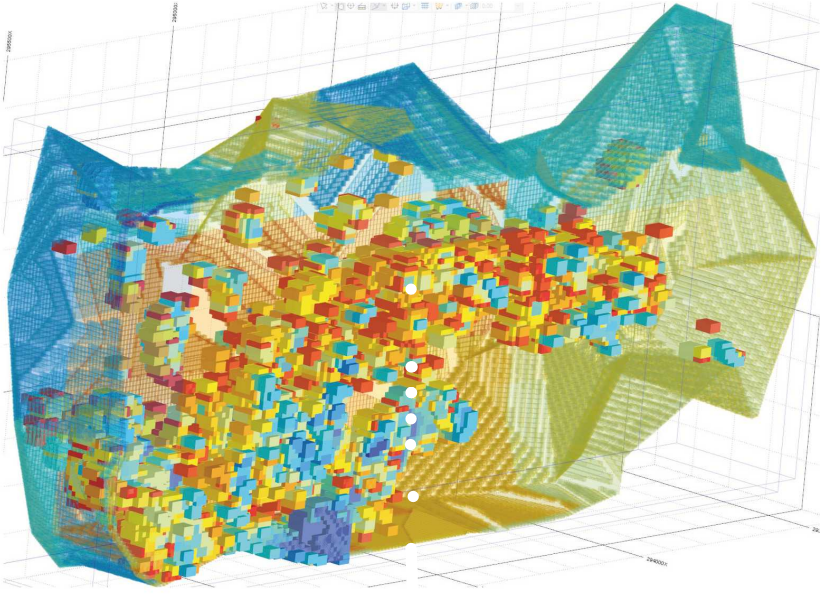
\includegraphics[width=0.6\textwidth]{assets/1250}
	\caption*{Рис. 1 -- Пример результата работы первого алгоритма для мощного рудного тела}
	\caption*{Второй алгоритм «Комбинация частей, полученных по заданной сетке»}
\end{figure}

\begin{multicols}{2}
Если рассмотреть в поперечном сечении направление очистных работ,
некоторые системы разработки подразумевают формирование выемочных единиц
по регулярной сети. В то время как первый инструмент определяет
оптимальные координаты выемочных единиц с учетом заданного минимального
размера и формы, новый подход позволяет задать требования к форме
поперечного сечения относительно двумерной сетки, а также к ее положению
и ориентации относительно рудного тела. Затем данный инструмент
проецирует выемочные единицы из ячеек сетки нарудное тело и разделяет
его на тонкие части (срезы), для которых определяется экономическая
оценка {[}4{]}. Используя минимальную и максимальную длину выемочной
единицы, параметры разделения, а также параметры ближней и дальней зоны
разубоживания, алгоритм поиска решений комбинирует ранее созданные части
таким образом, чтобы сформировать выемочную единицу, удовлетворяющую
заданной оценке или требуемому содержанию{[}5{]}.

В отличие от первого алгоритма, для которого степень детализации
выемочной единицы определяется размерами блоков регуляризированной
блочной модели, второй работает с каркасами, нарезая блоки в
соответствии с параметрами выемочных единиц, границами рудного тела и
зонами исключения. В результате степень детализации выемочной единицы
соответствует мощности одного среза, которую можно задать (рисунок 2,3).
Таким образом, второй алгоритм хорошо подходит для детального
проектирования {[}6{]}.
\end{multicols}

\begin{figure}[H]
    \centering
    \begin{subfigure}[b]{0.45\textwidth}
        \centering
        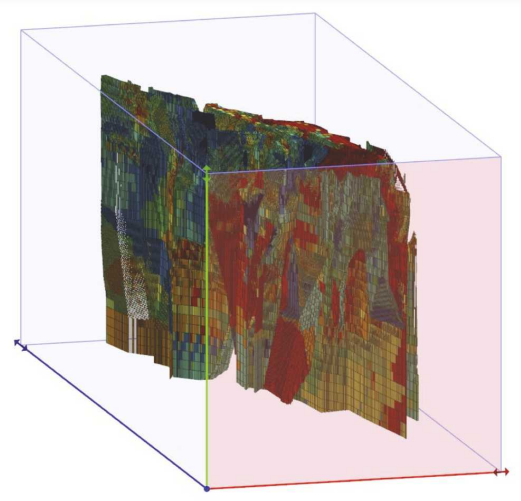
\includegraphics[width=\linewidth]{assets/1251}
		\caption*{Рис. 2 -- Интерактивное размещение границ сетки для второго алгоритма}
    \end{subfigure}
    \hfill
    \begin{subfigure}[b]{0.45\textwidth}
        \centering
        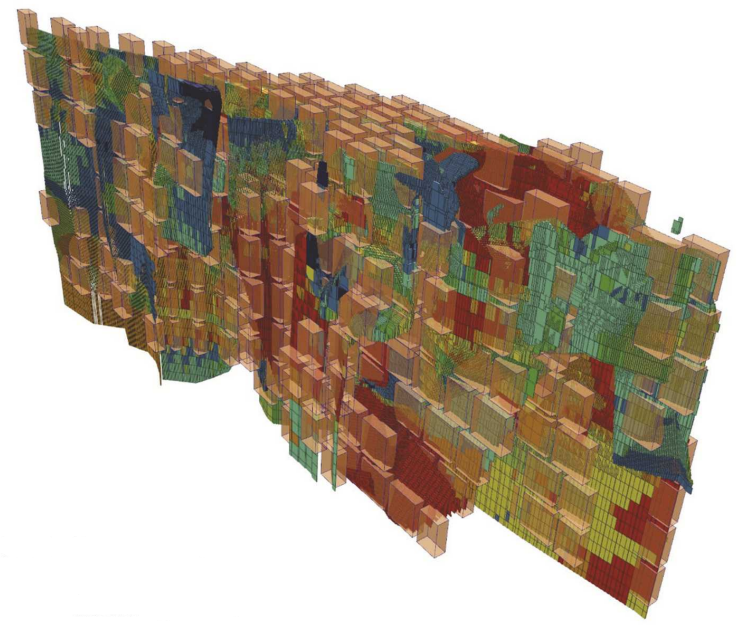
\includegraphics[width=\linewidth]{assets/1252}
		\caption*{Рис. 3 -Пример результата работы второго алгоритма для жильного рудного тела}
    \end{subfigure}
\end{figure}

\emph{Рабочий процесс оптимизации ВЕ. Параметры оптимизации(рудник).}
Для оптимизации необходимо использовать функцию Оптимизация выемочных
единиц на ленте Горные работы (рисунок 4).

\begin{figure}[H]
	\centering
	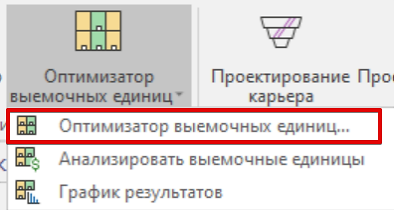
\includegraphics[width=0.5\textwidth]{assets/1253}
	\caption*{Рис. 4 - Функция Оптимизация выемочных единиц}
\end{figure}

Далее необходимо настроить параметры оптимизации на трех вкладках
Рудник, Переработка и Потребители. Если Вы производите оптимизацию по
бортовому содержанию, то заполняется только вкладка Рудник (рисунок 5).

\begin{figure}[H]
	\centering
	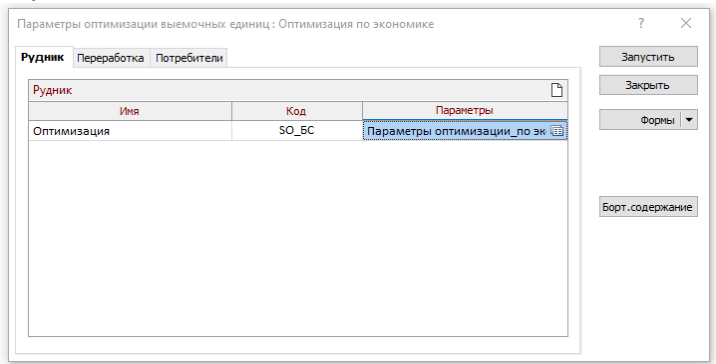
\includegraphics[width=0.8\textwidth]{assets/1254}
	\caption*{Рис. 5 - Параметры оптимизации}
\end{figure}

\begin{multicols}{2}
Имя: Введите название месторождения, по которому вы будете выполнять
оптимизацию.

Код: Введите идентификационный код, который будет присвоен
месторождению. Этот код будет использоваться для идентификации
месторождения в отчетах.

Параметры: Необходимо создать или выбрать существующий набор форм с
параметрами оптимизации.

\emph{Вкладка блочная модель}

На вкладке необходимо выбрать блочную модель, определить её Тип. Если
блочная модель рудная Вы можете ограничить оптимизацию ЦМП или
координаторами. При использовании полной БМ ограничения будут получены
из блочной модели. В выемочных единицах, которые будут частично
находиться за пределами полной БМ, расчеты показателей будут только по
той части, которая внутри БМ (рисунок 6).
\end{multicols}

\begin{figure}[H]
	\centering
	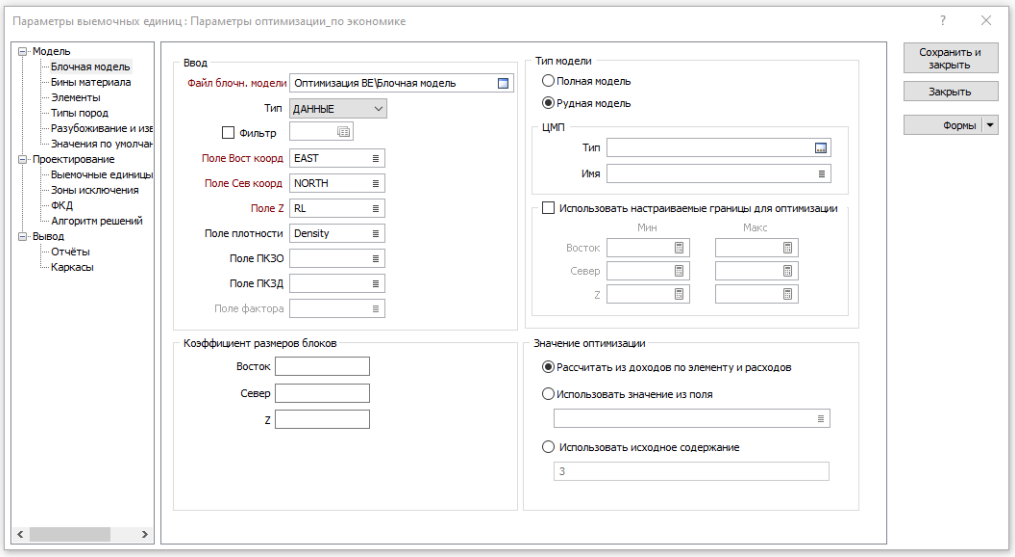
\includegraphics[width=0.8\textwidth]{assets/1255}
	\caption*{Рис. 6 - Вкладка блочной модели}
\end{figure}

\begin{multicols}{2}
\emph{Поле ПКЗО}

Поправочный коэффициент затрат на обогащение определяет только те
затраты, которые будут понесены, если руда пройдет переработку на
обогатительной фабрике. Эти затраты вводятся в виде фактора относительно
"стандартного блока", который имеет поправочный коэффициент на затраты
на обогащение, равный 1.

\emph{Поле ПКЗД}

Поправочный коэффициент затрат на добычу определяет только те затраты,
которые будут понесены, если блок будет добыт. Затраты, не учитываемые
при остановке добычных работ, не влияют на коэффициент поправки для
добычных работ. Эти затраты вводятся в виде фактора относительно
"стандартного блока", который имеет поправочный коэффициент затрат на
добычу, равный 1.

Если это поля ПКЗД и ПКЗО оставлены пустыми, либо значения в указанных
полях отсутствуют, тогда будет применяться значение по умолчанию,
заданный во вкладке Значения по умолчанию.

\emph{Поле факторов}

Если вы используете факторную модель для оптимизации, укажите имя поля,
которое содержит фактор для каждого блока модели.

Методы определения значения оптимизации (рисунок 7):
\end{multicols}

\begin{figure}[H]
	\centering
	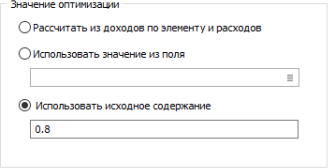
\includegraphics[width=0.5\textwidth]{assets/1256}
	\caption*{Рис. 7 -- Значение оптимизации}
\end{figure}

\begin{multicols}{2}
\emph{Рассчитать из доходов по элементу и расходов}

Выберите эту опцию, чтобы вычислить значение оптимизации для каждого
блока из заданных экономических параметров.

Значение каждого рудного блока (доход от элемента - затраты на
переработку - затраты на добычу руды - затраты на извлечение элемента -
затраты на продажу) сравнивается со значением породы (то есть стоимость
добычи пустой породы) для всех методов переработки. Если денежный поток
руды больше денежного потока пустой породы, тогда элементы материала
обрабатываются как РУДА. В противном случае элементы обрабатываются как
ПОРОДА.

\emph{Использовать значение из поля}

Выберите поле блочной модели, в котором будет предварительно рассчитаны
значение оптимизации (разница между доходом и расходом).

\emph{Использовать исходное содержание}

В данном случаи задается бортовое содержание. В итоговых ВЕ содержание
будут больше или равно заданному значению.

\emph{Вкладка Бины материала.} На данной вкладке задаются добываемые
материалы, например сорта руды. Данная вкладка является необязательной
для заполнения. Если вы не хотите как-либо классифицировать ваши
материалы, вы можете оставить ее пустой.

\emph{Вкладка Элементы.} На вкладке Элементы задаются элементы из
блочной модели, которые будут участвовать в процессе переработки.

\emph{Вкладка Разубоживание и извлечение.} На данной вкладке необходимо
указать значения потерь и разубоживания. Значение можно задавать в
факторах или процентах.

\emph{Разубоживание.} Разубоживание выражается как в ФАКТОРАХ, так и в
ПРОЦЕНТАХ. Если вы используете фактор, то введите значение, которое
больше или равно 1. Значение 1 -- нет разубоживания. Фактор
разубоживания показывает, какое количество пустой породы будет добыто
вместе с рудой. Данный коэффициент влияет на добытый объем по всем
блокам. Другими словами, если объем блока равен 100, разубоживание равно
1.2, тогда переработанный объем будет равен 120, а содержания полезного
компонента соответственно разубожены. Чтобы преобразовать проценты в
факторы, необходимо сделать следующее вычисление (ПРОЦЕНТЫ / 100) + 1.
Если разубоживание равно 50\%, тогда значение фактора равно 1.5.

Укажите Поле извлечения/потерь, если вы хотите использовать различные
значения извлечения для каждого блока вместо того, чтобы использовать
постоянное значение. Для расчета тоннажа добытой руды можно использовать
2 формулы:

\begin{enumerate}
\def\labelenumi{\arabic{enumi}.}
\item
  Порода/Руда
\end{enumerate}

Тоннаж добытой руды = Тоннаж руды в недрах × Извлечение ×
(1+Разубоживание)

\begin{enumerate}
\def\labelenumi{\arabic{enumi}.}
\setcounter{enumi}{1}
\item
  Порода/(Руда+ Порода)
\end{enumerate}

Тоннаж добытой руды =Тоннаж руды в недрах × Извлечение × 1

\emph{Извлечение/Потери.} Извлечение -- это величина обратная потерям
(то есть, если ваши потери, при извлечении из недр, составляют 10\%, то
извлечение составит 90\%). Введите значение Извлечения, которое больше
нуля и меньше или равно 1. Коэффициент извлечения показывает количество
руды, которое может быть извлечено из карьера и отправлено на
переработку. Он влияет на объем каждого блока. Единицы извлечения/потерь
могут быть выражены в ФАКТОРАХ или ПРОЦЕНТАХ. Например, если объем блока
равен 100, а фактор извлечения равен 0.9, это означает, что 90\% блока
может быть извлечено, а 10\% будет потеряно. Добытый и переработанный
тоннаж будет 90 (то есть 100 * 0.9) {[}7,8{]}.

\emph{Вкладка Значение по умолчанию.} Данная вкладка используется для
определения значений по умолчанию: Плотности, ПКЗО и ПКЗД для руды и
породы. Когда цена добычи и переработки изменяется на различных
горизонтах или ниже ЦМП, то изменяемые условия можно прописать во
вкладке Значения по умолчанию .

\emph{Вкладка Выемочные единицы.} Данная вкладка позволяет выбрать
алгоритм для создания выемочных единиц. Также здесь можно указать
области в виде каркаса или заданных координат, чтобы использовать для
них разные параметры выемочных единиц.

\emph{Параметры выемочных единиц.} В зависимости от выбранного
алгоритмам (метода) оптимизации формы диалогового окна Параметры
выемочных единиц будут отличаться. Рассмотрим параметры на примере
оптимизации методом срезов.

\emph{Вкладка Зоны исключения.} Здесь Вы можете исключить/обрезать
результаты оптимизации в пределах или за пределами выбранных каркасов
или контуров.

\emph{Вкладка Отчеты.} Позволяет настроить отчеты по выемочным единица
или по срезам, которые участвовали в оптимизации, для анализа
результатов. Также можно использовать функцию Генератор отчетов для
создания отчета пользовательской структуры и наполнений.

\emph{Вкладка Каркасы.} На вкладке каркасы необходимо указать Тип и Имя
(префикс имени) для итоговых выемочнх едениц. Также Вы можете создать
отдельно каркасы Ближней и дальней зоны разубоживания и каркасы с учетом
этих зон (выемочная еденицы) и без (ядро) (рисунок 8).
\end{multicols}

\begin{figure}[H]
	\centering
	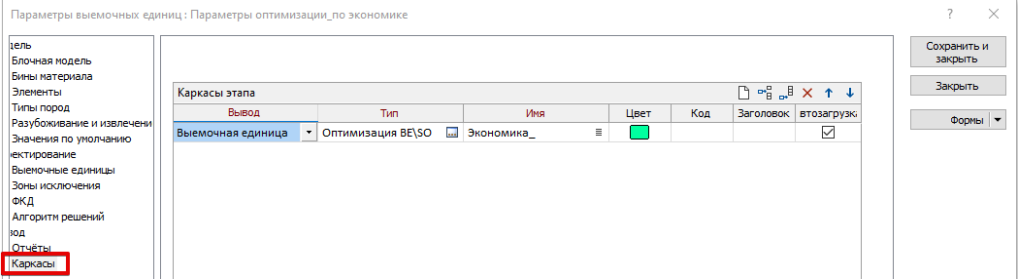
\includegraphics[width=0.8\textwidth]{assets/1257}
	\caption*{Рис. 8 - Функции каркаса}
\end{figure}

\begin{multicols}{2}
{\bfseries Результаты и обсуждение.} Так как настройки модулей «Оптимизатор
карьеров» и «Оптимизатор выемочных единиц» в MICROMINE практически
идентичны, достаточно освоить один из модулей, чтобы перейти к работе со
вторым. Кроме того, оба этих модуля используют встроенные в MICROMINE
алгоритмы поиска оптимальных решений, поэтому нет необходимостив
дополнительных финансовых вложениях в лицензии сторонних оптимизационных
решений {[}7,9{]}.

Описанные в статье инструменты оптимизации выемочных единиц используют
разные подходы к решению задачи, поэтому каждый из них имеет свои плюсы
и минусы.

Первый алгоритм, который формирует выемочные единицы из комбинации
материнских блоков, требует минимальных предварительных знаний об
оптимальных координатах расположения выемочных единиц, об ориентации
рудного тела или о системе разработки. Это делает его очень подходящим
для проектов «с нуля» и для выполнения технико-экономического
обоснования {[}10{]}. Он также подходит для определения внешних
экономических границ для больших рудных тел.

Второй алгоритм требует более глубоких знаний о структуре рудного тела и
предполагаемой системе разработки, что делает его более подходящим для
уже разрабатываемых месторождений и детального проектирования подземных
рудников. Кроме того, он дает более качественные результаты для жильных
рудных тел, чем первый, при использовании которого выемочные единицы,
вероятно, будут более грубыми.

{\bfseries Выводы.} Использование программного обеспечения MICROMINE для
оптимизации подземных выемочных добычных единиц открывает новые
возможности для улучшения эффективности горнодобывающих операций.
Экономический подход, сочетающий в себе уменьшение затрат, увеличение
добычи и минимизацию рисков, делает MICROMINE важным инструментом в
индустрии добычи полезных ископаемых. Решения, основанные на этом
программном обеспечении, могут существенно влиять на
конкурентоспособность предприятий в условиях постоянно меняющейся
горнодобывающей среды.
\end{multicols}

\begin{center}
{\bfseries Литература}
\end{center}

\begin{noparindent}
1. MICROMINE технологии нового поколения для горной добычи (Редакция от
07.07.2023) --URL:

https://www.micromine.kz/2023-5-release/ (Дата
обращения 09.01.2024)

2. Мигер К., Димитракопулос Р., Эйвис Д. Оптимизация метода
проектирования карьера, размера выемочных блоков и проблема межблочного
интервала //Физико-технические проблемы разработки полезных ископаемых.
- 2014. - № 3. - С. 96--117.

3. Капутин Ю.Е. Информационные технологии планирования горных работ //
Недра. -Санкт-Петербург, 2004. -- 334 с.

4. Должиков П.Н., Величко Н.М., Должикова А.П., Основы экономики и
управления горным предприятием: учебное пособие // Норд-пресс. -
Донецк.- 2009. -- 200 с.

5. Тонких А.И.и др. Технико-экономические расчеты при подземной
разработке рудных месторождений: учеб. Пособие. - Изд-во ДВГТУ,
Владивосток, 2007. -137 с.

6. Холл Брайан. Бортовые содержания и оптимизация стратегии Р85 горных
работ. Пер. с англ. -Правовед, Екатеринбург, 2017. - 380 с.

7.Уткина С.И. Экономика горного предприятия. -М: Изд-во Московского
государственного горного университета, 2003. - 262 с.

8. В. Мамлеев Планирование открытых горных работ в программе Micromine
Alastri.// Глобус.-2022.- № 3 (72).- С. 116-119

9. К. А. Филимонов В. А. Карасёв / Технология подземных горных работ--
{[}Электронный ресурс{]}: учебное пособие. -Кемерово, КузГТУ, 2013.-110
с.

10. Л. Н. Кузина, C.Ф. Богдановская, Ж.В. Миронова Экономика горного
производства:

Практикум. -Красноярск, Сиб. федер. ун-т, 2011. -140 с.
\end{noparindent}

\begin{center}
{\bfseries References}
\end{center}

\begin{noparindent}
1. MICROMINE tekhnologii novogo pokoleniya dlya gornoi dobychi
(Redaktsiya ot 07.07.2023) --URL:

https://www.micromine.kz/2023-5-release/ (Data obrashcheniya 09.01.2024)
{[}in Russian{]}

2. Miger K., Dimitrakopulos R., Eivis D. Optimizatsiya metoda
proektirovaniya kar\textquotesingle era, razmera vyemochnykh blokov i
problema mezhblochnogo intervala //Fiziko-tekhnicheskie problemy
razrabotki poleznykh iskopaemykh. - 2014. - № 3. - S. 96--117. {[}in
Russian{]}

3. Kaputin Yu.E. Informatsionnye tekhnologii planirovaniya gornykh rabot
// Nedra. -Sankt-Peterburg, 2004. -- 334 s. {[}in Russian{]}

4. Dolzhikov P.N., Velichko N.M., Dolzhikova A.P., Osnovy ekonomiki i
upravleniya gornym predpriyatiem: uchebnoe posobie // Nord-press. -
Donetsk.- 2009. -- 200 s. {[}in Russian{]}

5. Tonkikh A.I.i dr. Tekhniko-ekonomicheskie raschety pri podzemnoi
razrabotke rudnykh mestorozhdenii: ucheb. Posobie. - Izd-vo DVGTU,
Vladivostok, 2007. -137 s. {[}in Russian{]}

6. Kholl Braian. Bortovye soderzhaniya i optimizatsiya strategii R85
gornykh rabot. Per. s angl. -Pravoved, Ekaterinburg, 2017. - 380 s.
{[}in Russian{]}

7.Utkina S.I. Ekonomika gornogo predpriyatiya. -M: Izd-vo Moskovskogo
gosudarstvennogo gornogo universiteta, 2003. - 262 s. {[}in Russian{]}

8. V. Mamleev Planirovanie otkrytykh gornykh rabot v programme Micromine
Alastri.// Globus.-2022.- № 3 (72).- S. 116-119 {[}in Russian{]}

9. K. A. Filimonov V. A. Karasev / Tekhnologiya podzemnykh gornykh
rabot-- {[}Elektronnyi resurs{]}: uchebnoe posobie. -Kemerovo, KuzGTU,
2013.-110 s. {[}in Russian{]}

10. L. N. Kuzina, C.F. Bogdanovskaya, Zh.V. Mironova Ekonomika gornogo
proizvodstva:

Praktikum. -Krasnoyarsk, Sib. feder. un-t, 2011. -140 s. {[}in
Russian{]}
\end{noparindent}

\emph{{\bfseries Сведения об авторах}}

\begin{noparindent}
Ахметканов Д.К. - канд.техн.наук, ассоциированный профессор, Satbayev
University, г.Алматы, Казахстан, e-mail:
d.akhmetkanov@satbayev.university;

Тян Л.Е. -магистрант Satbayev University, г.Алматы, Казахстан, e-mail:
laura301201@mail.com;

Абен Е.Х. - канд.техн.наук, ассоциированный профессор, Satbayev
University, г.Алматы, Казахстан, e-mail: y.aben@satbayev.university;

Елузах М. - канд.техн.наук, ассоциированный профессор, Satbayev
University, г.Алматы, Казахстан, e-mail: m.yeluzakh@satbayev.university
\end{noparindent}

\emph{{\bfseries Information about the authors}}

\begin{noparindent}
D.Akhmetkanov -- Candidate of Technical Sciences, Associate Professor of
Satbayev University, Almaty, Kazakhstan, e-mail:
d.akhmetkanov@satbayev.university;

L.Tyan - undergraduate student Satbayev University, Almaty, Kazakhstan,
e-mail: laura301201@mail.com;

Абен Е.Х. - Candidate of Technical Sciences, Associate Professor of
Satbayev University, Almaty, Kazakhstan, e-mail:
y.aben@satbayev.university;

Елузах М. -Candidate of Technical Sciences, Associate Professor of
Satbayev University, Almaty, Kazakhstan, e-mail:
m.yeluzakh@satbayev.university
\end{noparindent}
